%********************************************************************
% Appendix
%*******************************************************
% If problems with the headers: get headings in appendix etc. right
%\markboth{\spacedlowsmallcaps{Appendix}}{\spacedlowsmallcaps{Appendix}}
\chapter{Modelo auxiliar de 3 nodos}\label{ch:3Nodos}

Con el objetivo de explorar y ganar entendimiento acerca de cómo transformar modelos discretos en modelos de Glass, se utilizó una red Booleana de tres nodos que había sido estudiada previamente por \citeauthor{Reka3Nodos2010} \citep{Reka3Nodos2010}. En ese trabajo se caracteriza por completo el comportamiento de dicha red discreta. Este modelo discreto es mostrado en la figura \ref{fig:red3reka}.

\begin{figure}[hbt]
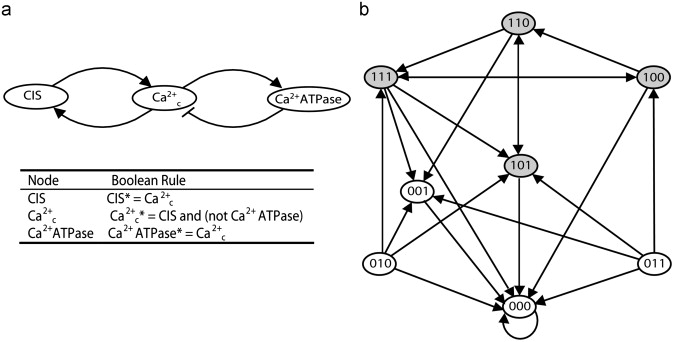
\includegraphics[width=0.9\linewidth]{gfx/red3nodos}
\caption[Modelo Booleano de 3 nodos]{Modelo Booleano de 3 nodos de \citeauthor{Reka3Nodos2010} \citep{Reka3Nodos2010}.\ a) Reglas L\'ogicas.\ b) Estados posibles de la red.}\label{fig:red3reka}
\end{figure}

Los nodos de esta red son $CIS$, $Ca^{2+}$ y $Ca^{2+}ATPase$

Las reglas lógicas de este modelo están dadas por:







%\begin{table}
%    \myfloatalign
%  \begin{tabularx}{\textwidth}{Xll} \toprule
%    \tableheadline{labitur bonorum pri no} & \tableheadline{que vista}
%    & \tableheadline{human} \\ \midrule
%    fastidii ea ius & germano &  demonstratea \\
%    suscipit instructior & titulo & personas \\
%    %postulant quo & westeuropee & sanctificatec \\
%    \midrule
%    quaestio philosophia & facto & demonstrated \\
%    %autem vulputate ex & parola & romanic \\
%    %usu mucius iisque & studio & sanctificatef \\
%    \bottomrule
%  \end{tabularx}
%  \caption[Autem usu id]{Autem usu id.}
%  \label{tab:moreexample}
%\end{table}
%
%Ei solet nemore consectetuer nam. Ad eam porro impetus, te choro omnes
%evertitur mel. Molestie conclusionemque vel at, no qui omittam
%expetenda efficiendi. Eu quo nobis offendit, verterem scriptorem ne
%vix.
%
%  
%\begin{lstlisting}[float,caption=A floating example]
%for i:=maxint to 0 do
%begin
%{ do nothing }
%end;
%\end{lstlisting}